\chapter{Aspecto organizacional}

\section{Introducci\'on}

Del relevamiento realizado en los talleres, se desprenden determinadas formas de organización interna, enmarcadas en las distintas realidades de los colectivos que las conforman, pero que comparten la gestion colectiva y la búsqueda de la horizontalidad en la toma de decisiones. Asimismo, la creación de la ley Nº 18.232 (Servicio Radiodifusión Comunitaria) provee el marco legal correspondiente, el cual genera una serie de derechos y obligaciones, que necesariamente condicionan de una forma u otra a la organización en sí misma.\\

Dentro de este marco legal, la ley considera a las Asociaciones Civiles sin fines de lucro con personería jurídica reconocidas por el Ministerio de Educación y Cultura o en trámite de constitución, también aquellos grupos de personas organizadas sin fines de lucro con iniciativas de carácter comunitario.\\

\section{Estructura (figura interna)}

\indent El estudio realizado permite dar cuenta de un universo diversificado en el cual conviven tanto sistemas organizacionales con estructuras claramente jerarquizadas (Asociación Civil) compuestas por directores, secretarios, coordinadores, tesoreros, etc; y otros con estructuras no tan elaboradas como las comisiones de vecinos. Si bien en una primera instancia se puede interpretar en el caso de las estructuras más complejas cierta rigidez, la información recabada también ha permitido entender que todas estas figuras que componen los diferentes organigramas organizacionales pretenden funcionar basados en la horizontalidad para la toma de decisiones. Cabe destacar que la capacidad referencial de ciertos integrantes de los colectivos ya sea por antigüedad, por saberes específicos, o por su capacidad de liderazgo funciona muchas veces como guía en la toma de decisiones del resto de los integrantes, lo que no significa que dichas decisiones no se pongan a consideración de la totalidad de colectivo.\\

En la mayoria de las radios comunitarias la organización interna dista de la figura legal, siendo más horizontales y flexibles que la forma jurídica que tienen que adoptar para existir legalmente. 
% Tanto las Asociaciones Civiles como las comisiones de vecinos son instrumentos de participación funcional, esta salvedad no es menor ya que justamente lo que muestra es el carácter de fluidez dentro de la organización, a saber, dichas estructuras no son respetadas a rajatabla en el funcionamiento sino más bien como una herramienta.

\section{Funcionamiento}

Se trabaja a través de asambleas ordinarias o extraordinarias en las cuales participa la totalidad del colectivo o en algunos casos los integrantes de la comisión directiva; donde se ponen en consideración los diferentes puntos a tratar. La periodicidad de dichas asambleas varía. Algunos colectivos realizan asambleas ordinarias de forma semanal, quincenal, mensual, otros una o dos veces al año. Lo mismo sucede con la elección de las distintas autoridades que componen tanto a las asociaciones como a las comisiones los tiempos varían. Las asambleas de carácter extraordinario se realizan según la urgencia a tratar.\\

Otra de las formas de funcionamiento es a través de la instrumentación de talleres compuestos por el equipo de trabajo donde se forman los espacios de decisión colectiva.\\

Las particularidades de cada colectivo son las que determinan el formato de funcionamiento. Un claro ejemplo se da en Radio Vilardevoz tanto en su estructura como en su forma de funcionamiento. Obviamente, se trata de un colectivo distinto, donde a pesar de la existencia de al menos tres modalidades de participación (como técnicos, usuarios del hospital o pasantes), se da una horizontalidad en las discusiones, que puede constatarse en la circulación de la palabra en las discusiones grupales.\\

\begin{figure}[htbp]
 \centering
 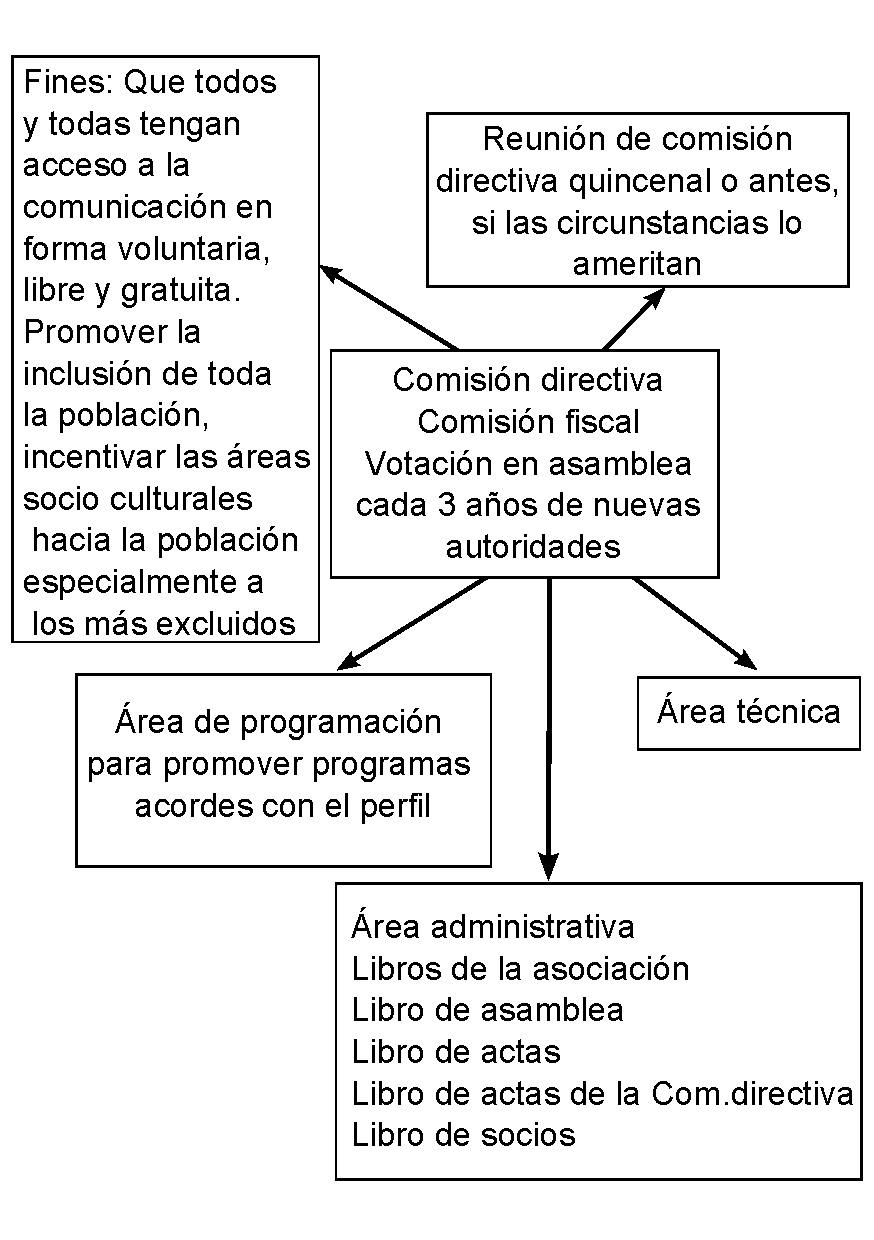
\includegraphics[scale=0.6]{./Cap/Organigramas/hela.pdf}
 % universo.pdf: 595x842 pixel, 72dpi, 20.99x29.70 cm, bb=0 0 595 842
 \caption{Organigrama de radio La Heladera, José Pedro Varela, Lavalleja.}
\end{figure}

\begin{figure}[htbp]
 \centering
 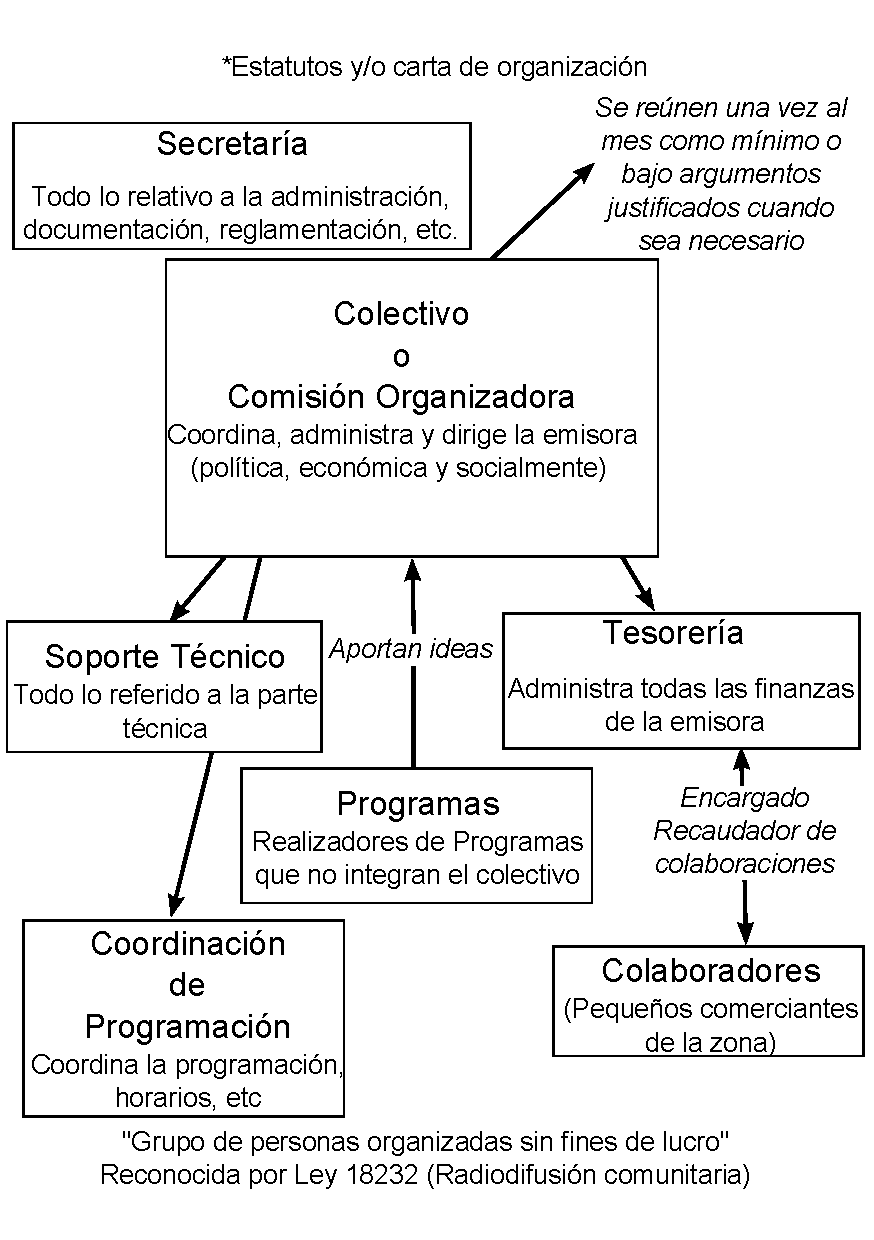
\includegraphics[scale=0.7]{./Cap/Organigramas/uni.pdf}
 % universo.pdf: 595x842 pixel, 72dpi, 20.99x29.70 cm, bb=0 0 595 842
 \caption{Organigrama de radio Universo, Montes, Canelones.}
\end{figure}

\begin{figure}[htbp]
 \centering
 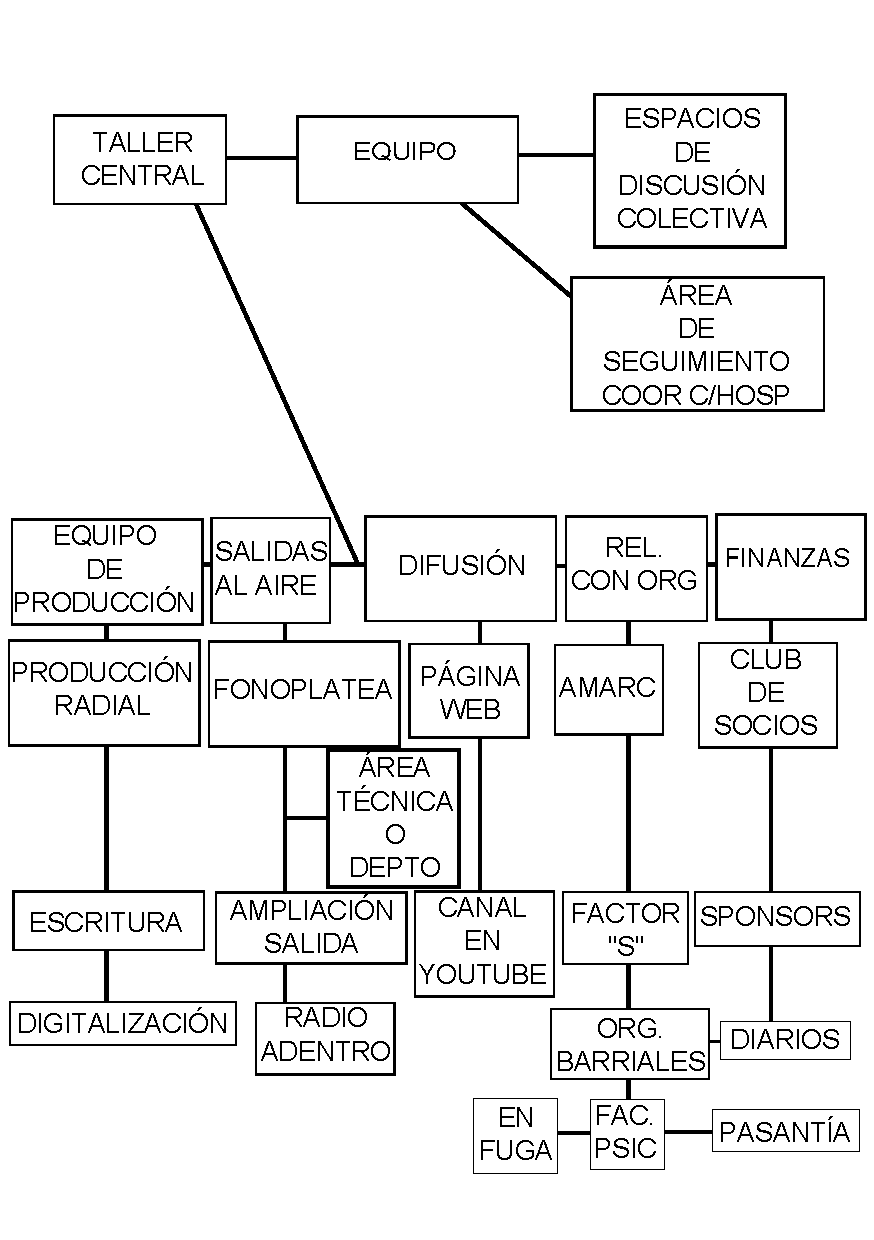
\includegraphics[scale=0.7]{./Cap/Organigramas/vilar.pdf}
 \caption{Organigrama de radio Vilardevoz, Montevideo.}
 \label{OrgVilardevoz}
\end{figure}
\newpage
\section{Elementos diferenciales}

Todas las organizaciones, tanto las asociaciones civiles como las comisiones de vecinos formadas presentan particularidades, innovaciones dentro de la estructura y por lo tanto formas de funcionamiento que se diferencian del resto y que de una u otra manera aportan al común de la red elementos diferenciales que podrían ser utilizados en beneficio de todos.\\

Algunos de estos elementos son los siguientes:\\

\textbf{Elaboración de Fines}\\

Estos fines refieren al compromiso del colectivo con la comunidad en las diferentes actividades que se realizan. Comunicación libre y gratuita, inclusión de los distintos proyectos radiales en la comunidad, actividades socioculturales, creación de espacios teatrales y musicales, etc.\\

\textbf{Inclusión de nuevos integrantes}\\

Se le provee a la persona que quiera ingresar al colectivo capacitación tanto técnica como en la propia elaboración de la propuesta radial. Asimismo se realiza un proceso de acompañamiento inicial, en el proceso de inclusión, que incluye un seguimiento del programa durante los primeros meses.\\

\textbf{Producción}\\

Se destacan los métodos de producción colectiva. Esto refiere a los contenidos tanto musicales como periodísticos con claros intereses referidos a la comunidad de la cual la radio es parte.\\

\textbf{Referentes}\\

La utilización de referentes por áreas permite un mejoramiento sustancial en las tareas diarias  ya sea en la parte técnica como en las tareas de producción radial, administrativas y de gestión.\\

\textbf{Figura de recaudador}\\

Algunas de las radios han optado por utilizar una persona que les facilite las cobranzas, tanto de la publicidad como de las cuotas sociales, que se utilizan para el financiamiento interno.\\

\textbf{Coordinadores de programación}\\

Permite integrar las grillas de programas. Trabaja en torno a los horarios y los tipos de programas que componen la grilla.\\